\documentclass{article}
\usepackage{a4wide}
\usepackage[utf8]{inputenc}
\usepackage[T1]{fontenc}
\usepackage[french]{babel}
\usepackage[babel=true]{csquotes} % guillemets français
\usepackage{graphicx}
\usepackage{color}
\usepackage{hyperref}
\hypersetup{colorlinks,linkcolor=,urlcolor=blue}

\usepackage{amsmath}
\usepackage{amssymb}

\title{Projet de développement mobile}
\author{Lebeau Olivier }
\date{April 2019}

\begin{document}

\maketitle
\begin{abstract}
Dans ce rapport, je décris la mise en place et le développement de mon projet. L'objectif de celui-ci étant de concevoir un jeu mobile sur Android et IOS.
\end{abstract}

\section{Introduction}
L'objectif étant de concevoir un jeu mobile, j'ai décidé de m'inspirer de jeux de shoot em up que je connais (Space Invaders,..).\\ 

Dans une première partie, je décrirais le fonctionnement globale de l'application. C'est à dire, quel est le but du jeu et comment y jouer. \\
Dans un second temps, je donnerons une description plus détaillée de l'application en décrivant l'architecture du code de manière globale d'abord puis plus spécifiquement sur android et IOS. \\
Et enfin, je m'attarderais sur les points que j'ai trouvé intéressant et les passages un peu plus délicats que j'ai rencontré lors de la conception de mon application. 
Dans ce rapport, les captures d'écrans du jeu sont réalisés sur la version android de l'application. \\


\tableofcontents

\newpage
\section{Description générale de l'application}

\begin{center}
  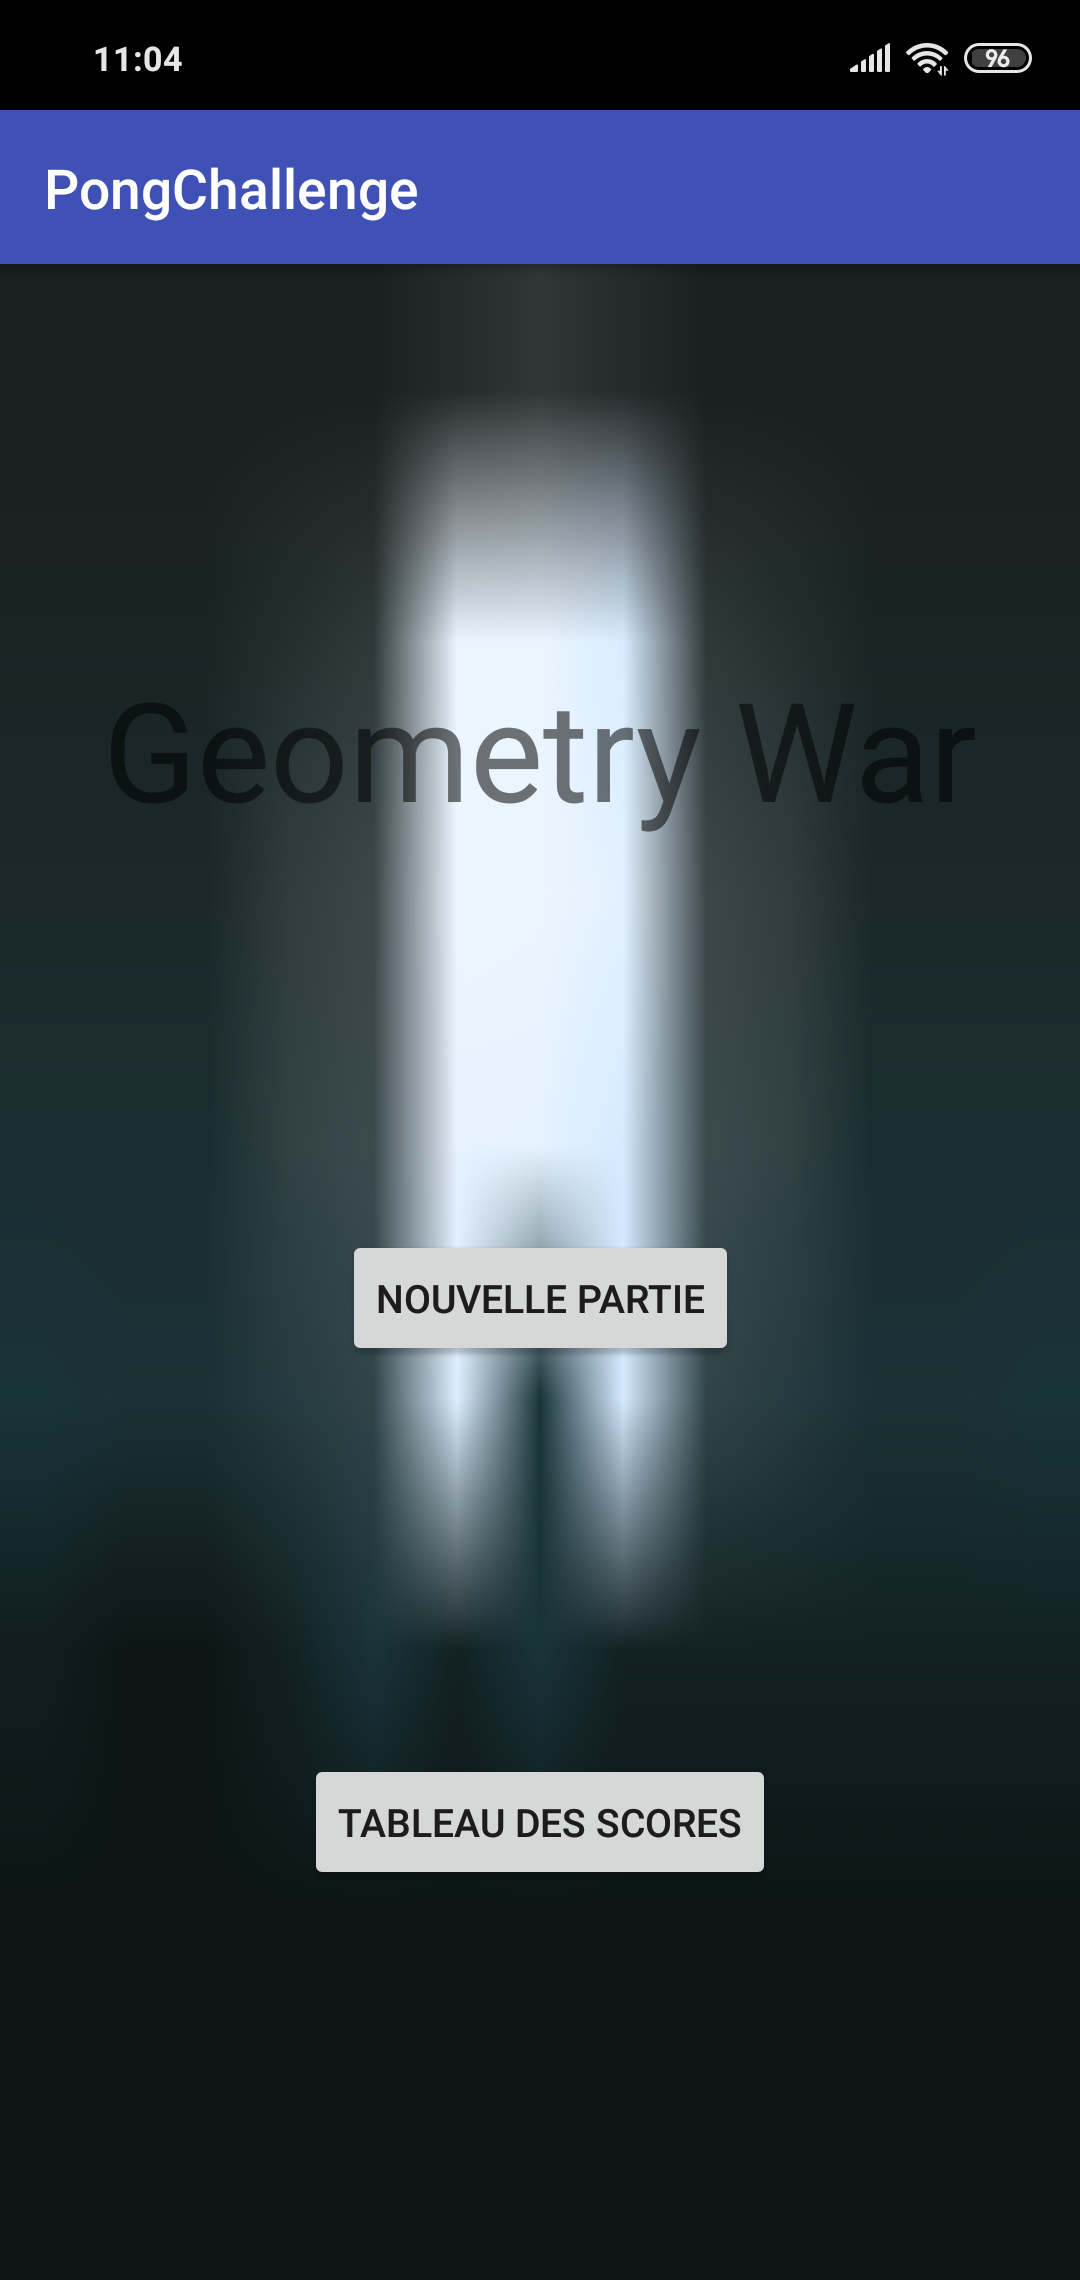
\includegraphics[scale=0.08]{Main.png}
  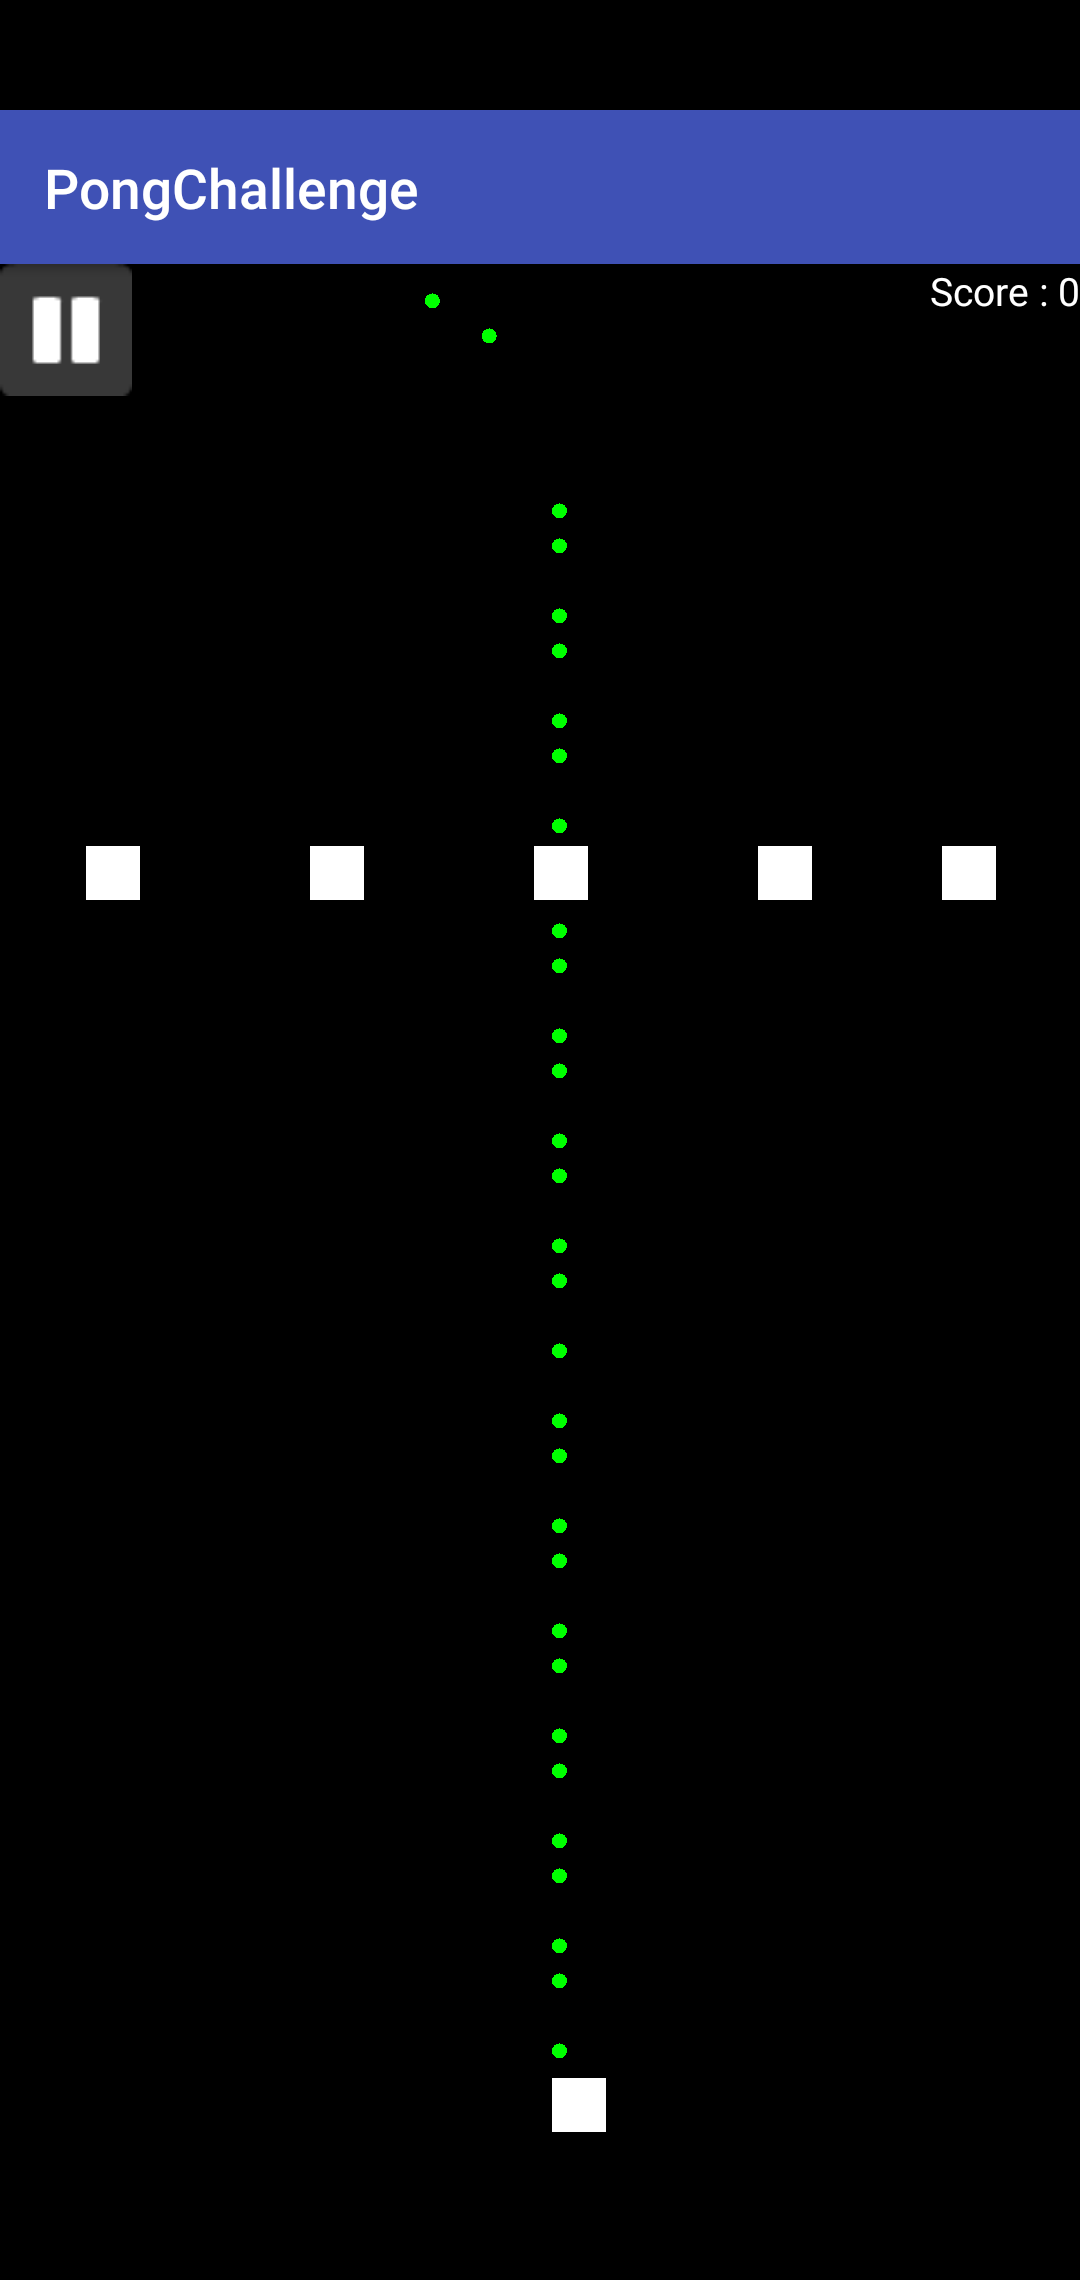
\includegraphics[scale=0.08]{Screenshot.png}
  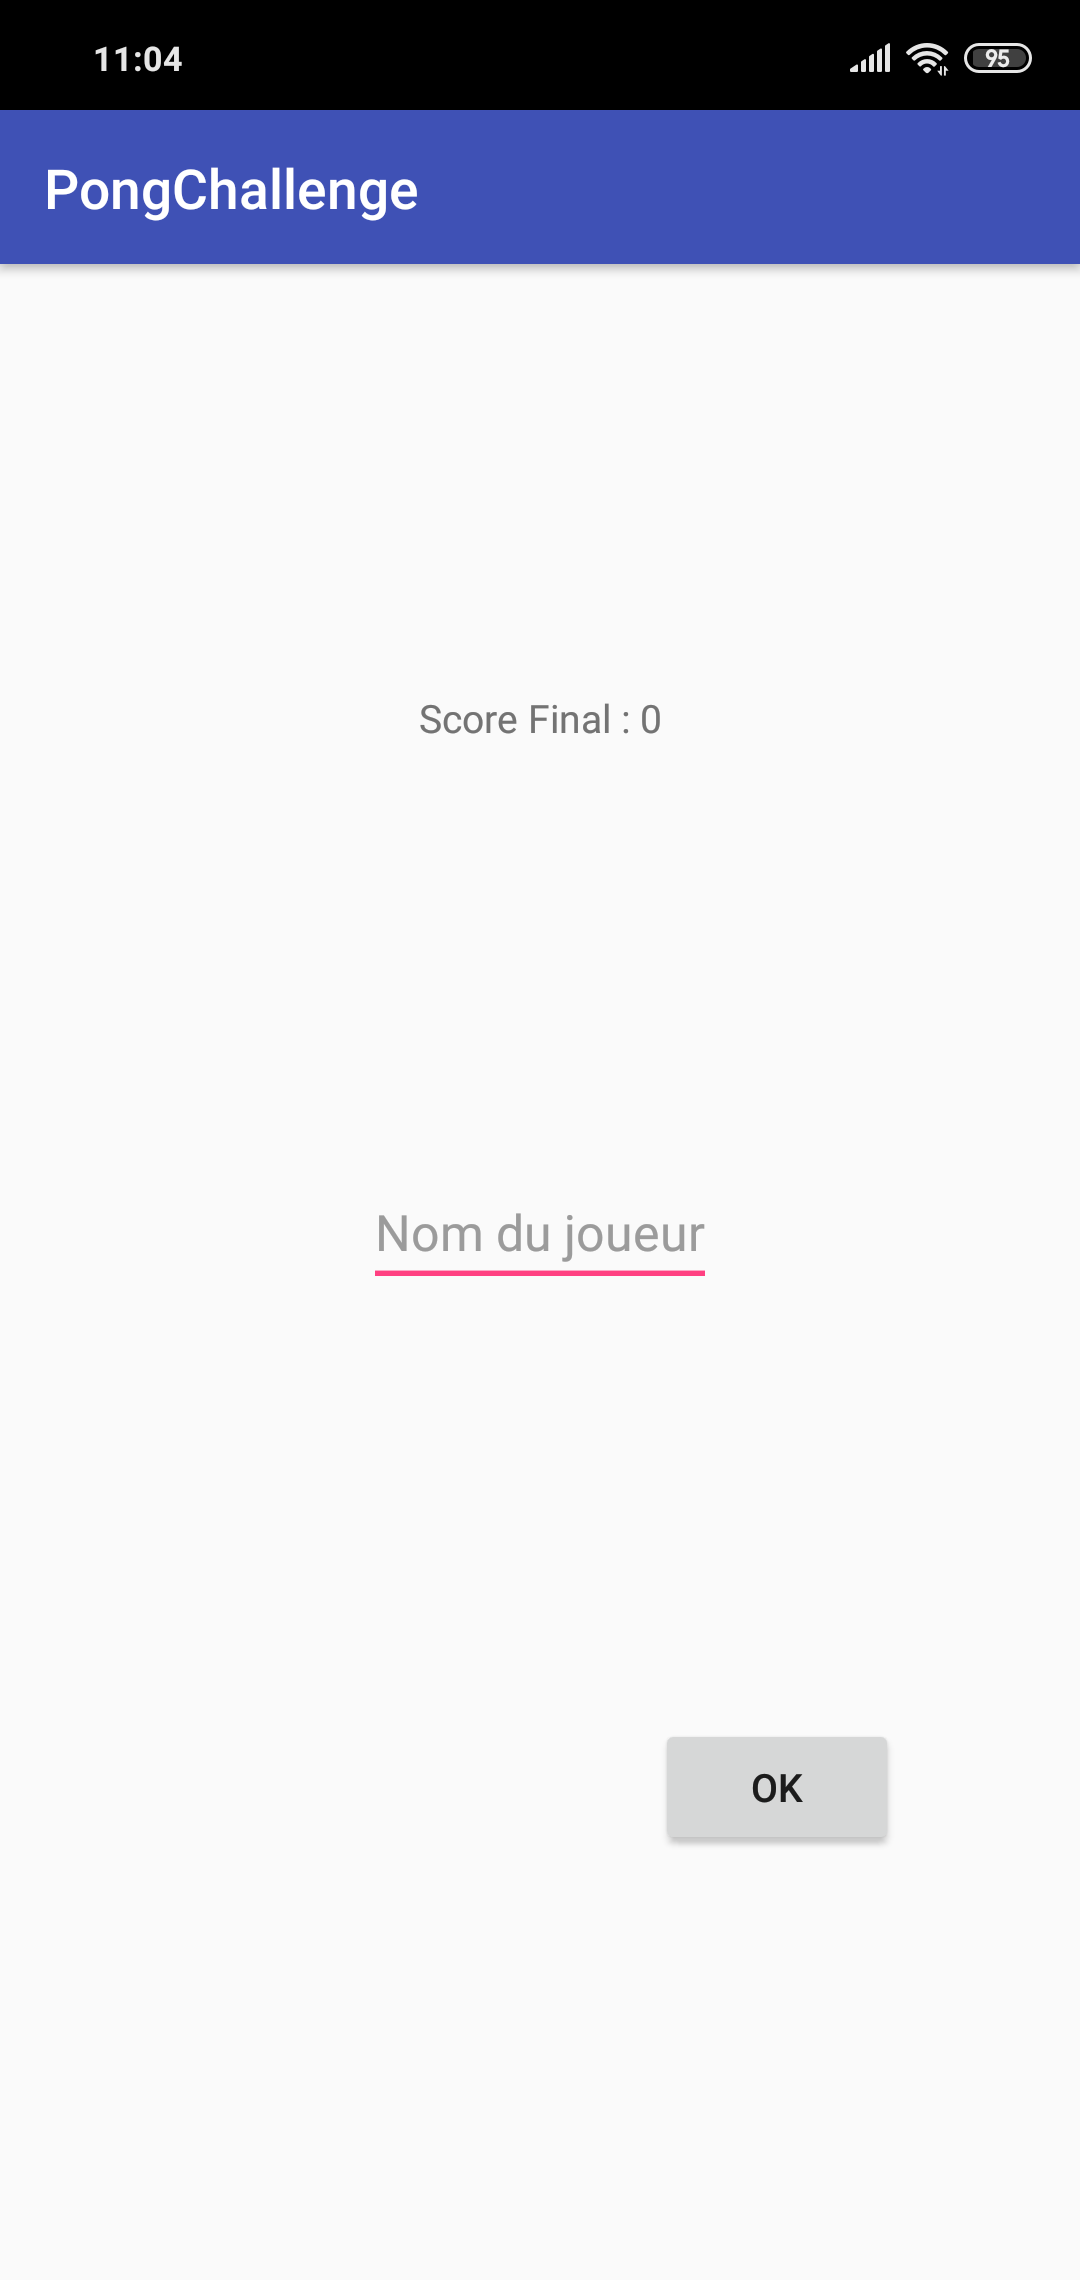
\includegraphics[scale=0.08]{screenAdd.png}
  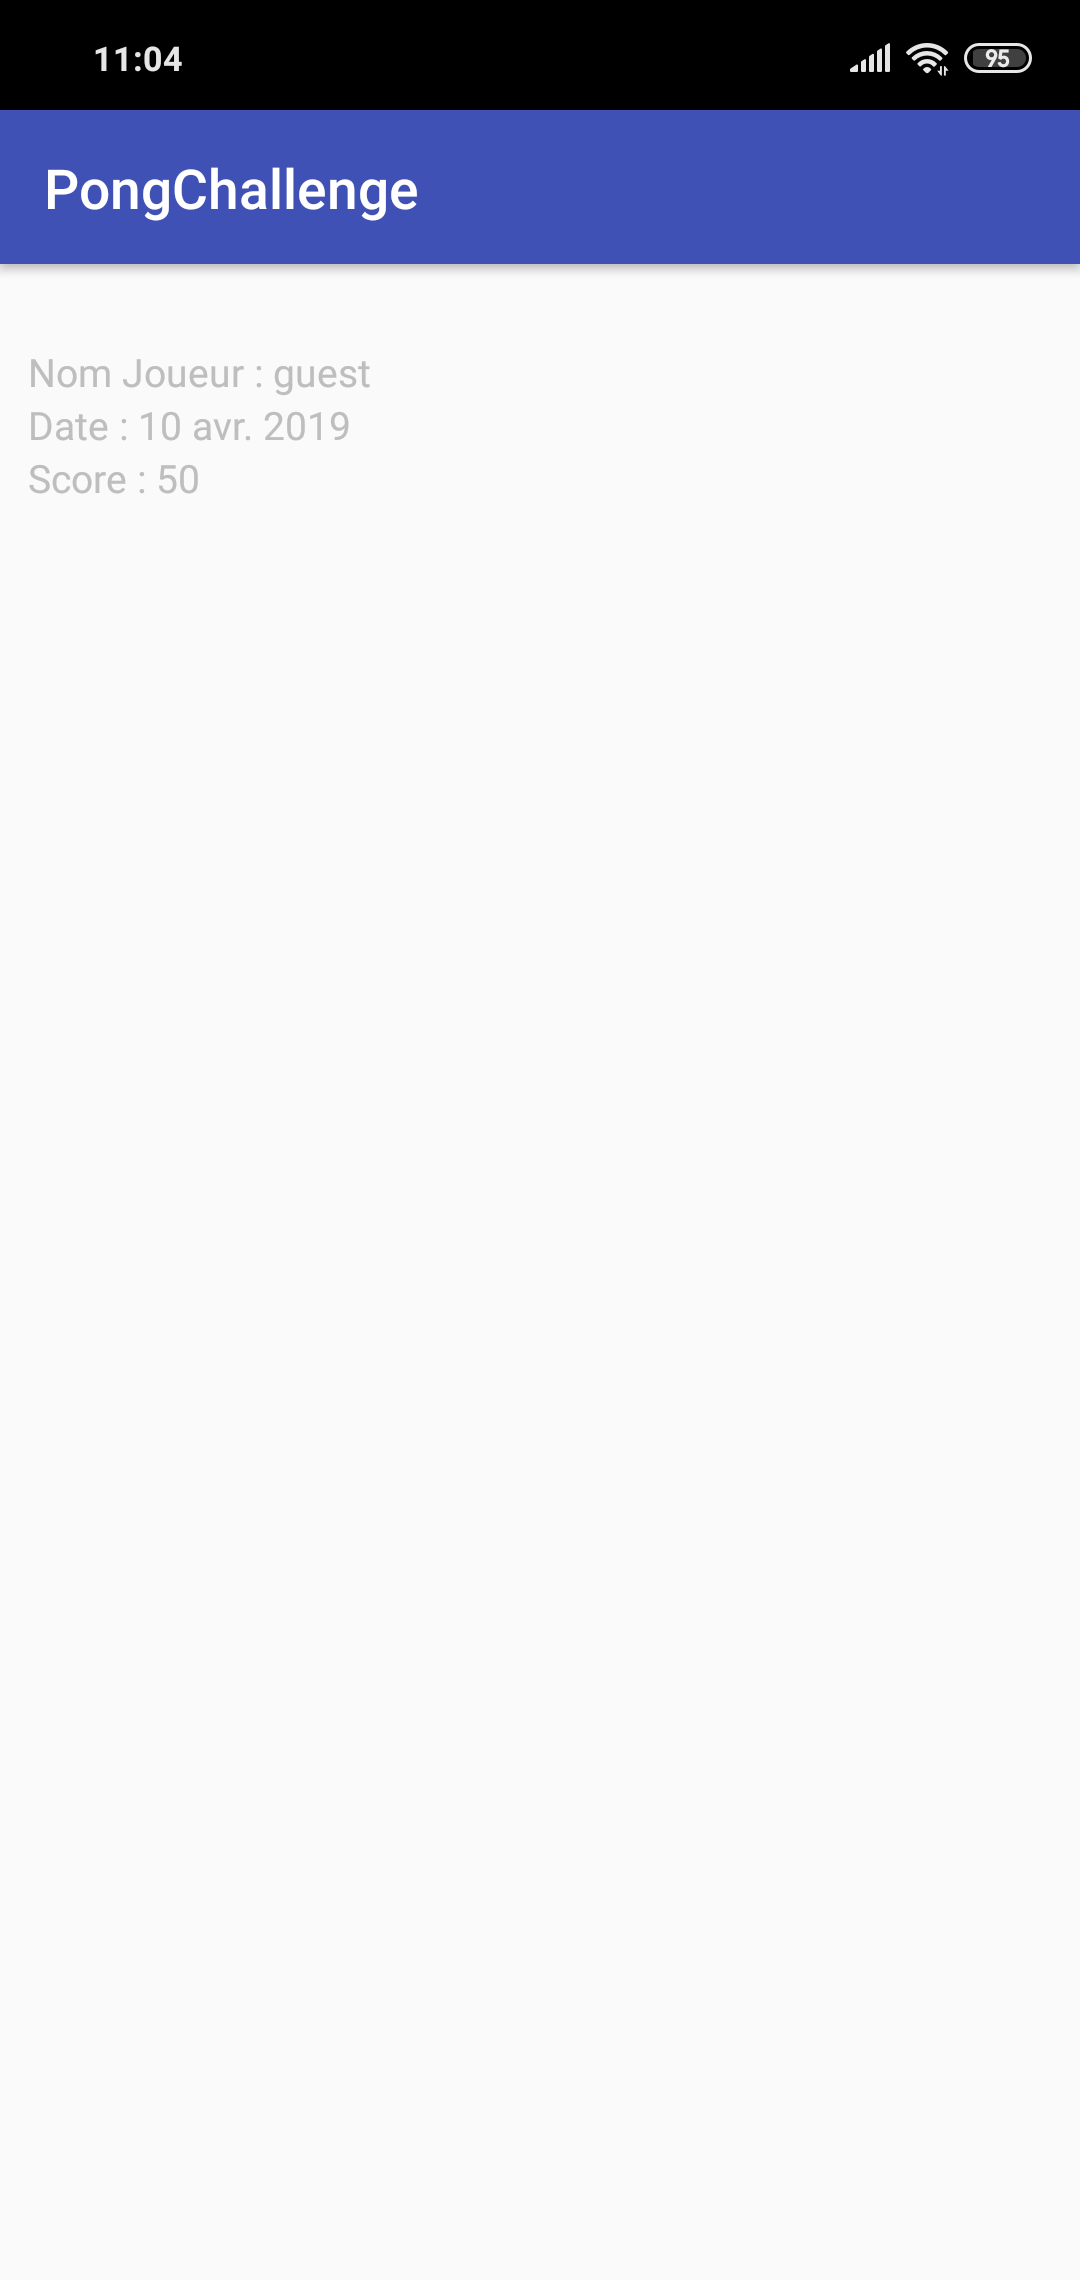
\includegraphics[scale=0.08]{ScreenScho.png}\\
    \caption{Fig1.Exemple d'écrans de jeu (Android)}
\end{center}
Le premier écran de jeu est le menu, à partir de celui-ci il peut soit jouer, soit accéder au tableau des scores. 
Supposons qu'il décide de jouer, arrive alors l'écran de jeu.
Le but du jeu consiste à tuer les ennemis tout en évitant les collisions avec les vagues successives.Chaque ennemi éliminé rapportant des points au joueur (Plus ou moins selon la valeur de l'ennemi). \\
De plus, lorsque le joueur avance dans la partie, les vagues d'ennemis générées contiennent de nouveaux ennemis qui adopte un comportement différent dans leurs déplacements. 
Si il y'a collision entre le joueur et un ennemi, le joueur a alors perdu sa partie. \\ 
Il arrive sur l'écran de saisie de pseudo qui lui permet d'ajouter un score et qui lui affiche le score obtenu pendant sa partie. Il peut choisir ou non d'enregistrer son score. \\ 
Il arrive à la fin sur le tableau des scores qui récapitule tout les scores. Si le joueur a décidé de ne pas sauvegarder son score, celui-ci est stocké en tant que score invité. 


\section{Architecture du code}
Malgré la différence de plateforme, afin de me faciliter la tâche j'ai voulu garder d'une manière globale la même architecture. 
\begin{center}
    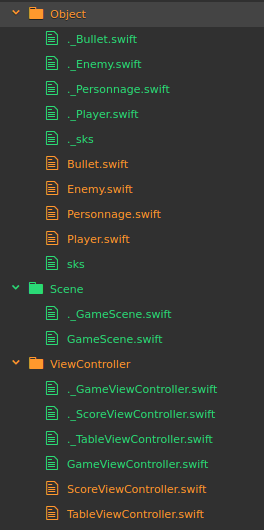
\includegraphics[scale=0.3]{ScreenIOS.png}
    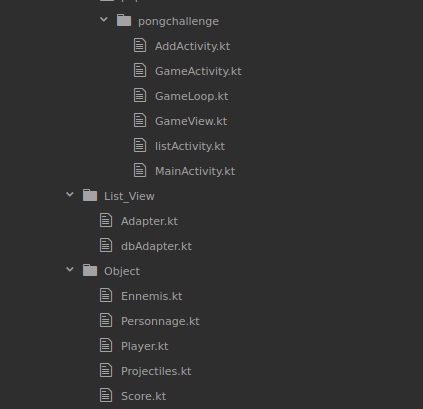
\includegraphics[scale=0.4]{AndroidArchi.png}
\end{center}
De ce fait, les objets utilisés dans le jeu sont dissociés des vues et des contrôleurs. \\ 
Ainsi dans les deux cas on a une classe Personnage dont hérite les classes Enemy et Player. Une classe pour la gestion des projectiles etc..\\

\subsection{Android}
Pour la conception du côté android, j'ai utilisé le langage \textbf{Kotlin} et l'IDE \textbf{Intellij Idea} qui embarque Android Studio \\
Si on regarde plus en détail notre version android, on voit que notre code est divisé dans 3 dossiers : 
\begin{itemize}
    \item pongChallenge : Contient les activités et la scène de jeu \\
    Pour faire cette application, j'ai utilisé une SurfaceView que j'ai intégré dans le layout game\_activity.xml. Cette vue personnalisée étant contenue dans la classe GameView.kt\\
    
    Dans ma classe GameView, celle-ci héritant de surfaceView il était nécessaire d'implémenter trois functions : 
    \begin{enumerate}
        \item surfaceCreated(holder: SurfaceHolder?) 
        \item surfaceChanged(holder: SurfaceHolder?, format: Int, width: Int, height: Int)
        \item surfaceDestroyed(holder: SurfaceHolder?)
    \end{enumerate}
    La première étant appelée lors de la création de la vue, la deuxième lors d'un changement dans celle-ci et la dernière lors de la destruction de notre vue.\\
    surfaceCreated(...) permet d'associer un Thread à notre gameView et de le démarrer : 
    \begin{verbatim}
    override fun surfaceCreated(holder: SurfaceHolder?) {
        if(loop?.state == Thread.State.TERMINATED) {
            loop = GameLoop(this)
        }

        loop?.setRunning(true)
        isRunning=true
        loop?.start()
    }
    \end{verbatim}
    On vérifie dans un premier temps qu'il n'y ait pas de Tread déjà actif, si il est bien terminé on en crée un nouveau qu'on récupère dans la variable loop et on le démarre. Ici j'ai aussi une variable isRunning que je passe à vraie dont nous parlerons plus tard. 
    Ce Thread contenu dans la classe GameLoop permet de faire boucler l'appel à deux fonctions de GameView : draw() et update() \\ 
    
    \begin{verbatim}
        override fun run() {
        //Déclaration des variables ...
        while(running){
            //traitements ....
            synchronized(view?.holder as Any) { view?.update() } //Mise à jour des déplacements
            //traitements ...
            var c:Canvas?=null
            try {
                c = view?.holder?.lockCanvas()
                synchronized(view?.holder as Any) { view?.draw(c as Canvas)}
            }finally {
                if(c!=null) view?.holder?.unlockCanvasAndPost(c)
            }
            //Traitements...
        }
    }
    \end{verbatim}
    J'ai gardé ici les deux passages qui nous intéresse, le premier est un appel à la méthode update() du gameView et le second montre les traitements mis en place pour dessiner l'écran de jeu avec la méthode draw(c as Canvas), l'objet Canvas étant l'objet permettant de dessiner dans notre vue.\\ 
    Ainsi notre interface de jeu est basée sur les méthodes draw() et update()\\
    
    Par conséquent, notre gameView contient ces deux méthodes.\\ 
    Pour la première : 
    \begin{verbatim}
    override fun draw(canvas: Canvas){
        super.draw(canvas)
        joueur?.projectiles?.forEach { i -> i.draw(canvas) }
        joueur?.draw(canvas,joueur?.posX as Float,(0.9f * hScreen as Int))
        wave?.forEach { i ->
            i.resize(wScreen as Int ,hScreen as Int )
            i.draw(canvas)
        }
    }
    \end{verbatim}
    Elle nous permet de dessiner les composants de notre jeu, à savoir, les projectiles du joueur, le joueur et les vagues d'ennemis. Les projectiles et les ennemis étant stockés dans des tableaux on parcourt donc ces tableaux et appel les méthodes draw interne à chaque objets. \\ 
    La méthode update quand à elle permet d'une part de déplacer les composants du jeu. Mais aussi de détecter les collisions entre les différents objets. Cette détection des collisions se faisant à l'aide de deux méthodes, une permettant de gérer les collisions projectiles ennemis : Algorithme de collision d'un point dans une box, et l'autre qui gère les collisions entre ennemis et joueur : Algorithme de collision pour deux box sur un plan 2D 
    \begin{verbatim}
        private fun collision(x:Personnage?,y:Personnage?):Boolean {
            /*
            Algorithme de Collision pour deux objets carrés (HitBox)
             */
            val Xx = x?.posX as Float
            val Xy = x.posY as Float

            val Yx = y?.posX as Float
            val Yy = y.posY as Float

            val yWidth = y.width    as Int

            val xWidth = x.width as Int
            val xHeight = x.height  as Int

            return (( (Yx < (Xx + xWidth) && Yx > Xx) || (Yx + yWidth > Xx)   && (Yx < Xx))
                            &&
                      ((Yy < (Xy + xHeight) && Yy > Xy)))
                    
    }
    \end{verbatim}
    Ici, en guise d'exemple la deuxième fonction de collision entre ennemis et joueur. \\ 
    Avec cette fonction on vérifie la collision à l'aide de hitbox représentant l'objet et on regarde si une des deux box a un point d'une de ses extrémités contenue dans l'autre objet.\\ 
    Les vagues venant exclusivement d'en haut je me suis contenté de vérifier la collision suivant l'axe Y que par le dessus du joueur.\\ 
    Le jeu va donc se dérouler de cette façon, la surface de jeu se lance ce qui a pour effet de générer un joueur, les ennemis et les projectiles. La génération d'ennemis se faisant dans la gameView de manière continue de manière assez basique, lorsqu'un ennemi meurt on en génére un nouveau à l'emplacement du tableau où se trouvait l'ancien ennemi. \\ 
    La génération des projectiles se fait quand à elle par le biais de la méthode attack() contenue dans la classe Player.kt : 
    \begin{verbatim}
    override fun attack() {
        runnable = object : Thread() {
            override fun run() {
                while(isAttack as Boolean) {
                    if ((projectiles?.size as Int) < 50) {
                        addQueue()
                    } else {
                        synchronized(this) {
                            for (i in 0 until projectiles?.size as Int) {
                                if (!(projectiles?.get(i)?.isActivate() as Boolean) 
                                ||projectiles?.get(i)?.hasHit() as Boolean) {
                                    projectiles?.set(i, generateProjectile())
                                    sleep(50)
                                }}}}}}
            fun addQueue(){
                synchronized(this) {
                    projectiles?.add(Projectiles(posX as Float, posY as Float,false))
                }}}
        runnable.start()
    }
    \end{verbatim}
    On crée un Thread qui va tout le long de la partie lorsque le joueur attack ajouter des projectiles au tableau contenu dans la classe Player.kt si le nombre de projectiles n'est pas égale à 50. Ou si ce nombre est atteint générer un nouveau projectile si un projectile a déjà touché un ennemi ou quitter l'écran de jeu.\\ 
    Le projectile ainsi généré se trouve à la position du joueur et se déplace dans la méthode update() du gameView() \\ 
    Pour finir, lorsque le joueur subit une collision, la partie se termine et on change d'Activity dans le but d'ajouter le score de la partie qui vient de se finir. \\
    On génère donc un intent comportant un attribut add qui est un boolean comportant une valeur true et le score de la partie qu'on envoie dans notre classe listActivity.kt qui gère notre tableau des scores. \\
    On déclenche ainsi le traitement suivant : 
    \begin{verbatim}
          if(intent.getBooleanExtra("Add",false)){
            val score = intent.getIntExtra("score",0)
            val intent = Intent(this,AddActivity::class.java)
            intent.putExtra("Score",score)
            startActivityForResult(intent,add)
        }
    \end{verbatim}
    
    Ce qui nous redirige vers l'activité AddActivity qui nous permet de récupèrer le nom du joueur. ayant utilisé la méthode startActivityForResult(..,..) après validation on retourne dans listActivity qui récupère le code résultat de startActivityForResult et soit ajoute le joueur dans la base de données, soit termine l'activité.
    
    \item List\_View : Contient les adaptateurs pour la base de données et la configuration des cellules du tableau des scores. Dans ce dossier nous avons donc la classe Adapter et la classe dbAdapter. \\
    Adapter est dotée d'une seule méthode (hormis son constructeur) qui est getView(..) qui nous permet de remplir les cellules de notre tableau avec un nom de joueur, un score et une date. 
    dbAdapter quand à elle contient toutes les méthodes permettant la communication avec la base de données dans laquelle les scores sont stockées. 
    \item Object : Contient les objets nécessaires au fonctionnement du jeu.
    Dans ce dossier nous avons par exemple les classes correspondant au joueur et aux ennemis, ces classes étant des spécialisation de la classe Personnage qui possède les attributs et méthodes que ces deux classes ont en commun. 
\end{itemize}

\subsection{IOS}
Hormis l'architecture similaire à celle utilisée pour la version android, les procédés mis en oeuvre diffèrent. \\
Pour la version IOS, j'ai utilisé pour l'interface de jeu le Framework SpriteKit. \\ 
Par conséquent, l'interface de jeu est désignée comme une scène que j'ai appellé ici GameScene. C'est dans celle classe que tout les traitements du jeu même sont décrits. A savoir, les déplacements des objets d'une parte dans la méthode update(...) et la gestion des collisions d'autre part dans la méthode didBegin(...). \\ \\
Ainsi au lancement du jeu, après être passé par le menu, on arrive sur l'interface de jeu qui se lance et génère le joueur et autres. Contrairement à android, chaque éléments de l'interface est désigné comme un noeud qui possède plusieurs attributs (Par exemple l'attribut physics qui désigne le comportement du noeud : Notamment dans les collisions).\\ 
Les ennemis et les projectiles sont générés dans la fonction startNewLevel() qui lance les actions (procédés propres à SpriteKit) qui sont des processus qui vont se dérouler sur l'interface de jeu.
\begin{verbatim}
       //génére les ennemis
        let spawnE = SKAction.run {
            let espace = self.gameArea.maxX/5
            for i in self.enemyArray{
                if !i.isAlive{
                    i.setPv(nb: 100+i.typeEnemy*50)
                    let startPoint = CGPoint(x: 5+CGFloat(i.indexTab)*espace,
                    y: self.size.height * 1.1)
                    
                    i.getNode().position = startPoint
                    i.typeEnemy = self.setType()
                    i.isAlive = true
                    self.addChild(i.getNode())
                }
            }
        }
        let spawSequence = SKAction.sequence([waitToSpawn,spawnE])
        let spawnForever = SKAction.repeatForever(spawSequence)
        self.run(spawnForever)
\end{verbatim}
Ici, on peut voir les traitements mis en place pour la génération des vagues d'ennemis via une SKAction personnalisé qui régénère des ennemis lorsque ceux-ci sont considérées comme mort.\\ 
Par la suite, via la méthode update(..) les ennemis, les projectiles vont se déplacer sur l'interface de jeu via leurs méthodes de déplacements respectives définis dans leur classe. La méthode update est donc constituée comme ceci : 
\begin{verbatim}
  override func update(_ currentTime : TimeInterval){
        if(gameState){
            if !enemyArray.isEmpty {
                for i in enemyArray{
                    if(i.isAlive){
                        i.move(ecranSize: self.size, posJoueur: player.getNode())
                        i.attack()
                    }
                }
            }
            if !bulletArray.isEmpty{
                for i in bulletArray{
                    if(i.isActivate){
                        i.move(size: self.size)
                    }
                    if i.hasHit{
                        i.isActivate=false
                        i.hasHit=false
                    }
                }
            }
        }else{
            endScene()
        }
    }
\end{verbatim}
gameState étant une variable permettant de définir si on est en jeu ou non.\\ 
On parcourt donc les tableaux d'ennemis et de projectiles et on fais déplacer les éléments si il sont vivants et/ou actifs. \\
Si on considère que le joueur perd, la valeur de gameState passe alors à false et on déclenche la méthode endScene() qui spécifie les traitements à mettre en oeuvre pour fermer l'interface de jeu : la destruction de la scene et le passage à l'écran d'ajout de score avec le contrôleur ScoreViewController qui nous permet d'afficher au joueur le score final et de récupérer un nom de joueur en vue de l'enregistrer dans le tableau des scores de TableViewController. \\ 
Puisqu'on utilise la persistance des données, on récupère dans ScoreViewController lors de l'enregistrement l'objet permettant de gérer les données à partir de TableViewController. Avec celui-ci on ajoute un nouveau score.\\ 
Contrairement à android j'ai pu externaliser le traitement de sauvegarde n'utilisant la TableView simplement pour l'affichage. \\
Ci-dessous la récupération dans le tableView du context de sauvegarde des scores. 
\begin{verbatim}
        if segue.identifier == "AddScore"{
            let controller =
                ((segue.destination as! UISplitViewController).viewControllers[1] as!
                UINavigationController).topViewController as! TableViewController
            
            let context = controller.fetchedResultsController.managedObjectContext
\end{verbatim}

\section{Points délicats/Intéressants}
Point délicats : 
\begin{itemize}
    \item 
La gestion des projectiles dans le jeu. En effet, sur la version android, le passage par un Thread a été une solution que j'ai trouvé afin d'envoyer les projectiles en continu sans avoir de ralentissements notable dans le jeu.
    \item 
La gestion des animations et images sur IOS étant plus simples j'ai pu contrairement à la version android incorporés des images dans le jeu. 
\end{itemize}

Point intéressants : 
\begin{itemize}
    \item La communication entre la gameScene et son contrôleur sur IOS a nécessité l'emploi d'un delegate que j'ai appelé GameViewControllerDelegate. Par cela, on utilise les fonctions du GameViewController dans la gameScene comme par exemple à la fin de la partie lorsqu'on doit faire passer le score à la vue d'ajout de score en utilisant AddScore(..) dans endScene(..)
    \begin{verbatim}
        func addScore(val:Int){
        let appDelegate = UIApplication.shared.delegate as! AppDelegate
        guard let storyboard = appDelegate.window?.rootViewController?.storyboard
        else {
            return
        }
        //Instantion du controller de vue ScoreViewController 
        let vc = storyboard.instantiateViewController(withIdentifier: "AddScoreView") as? ScoreViewController
        vc?.finalScore = val
        self.present(vc!, animated : true, completion : nil)
    }
    \end{verbatim}
\end{itemize}


\section{Conclusion}
Malgré le fait que la finalité soit la même lors de la conception sur une ou l'autre plateforme, les moyens mis en oeuvre sont différents apportant chacun leur lot de forces et de faiblesse.\\
D'un côté la mise en place du jeu sur IOS par l'utilisation de SpriteKit permet la mise en place plus simple de l'interface de jeu et de la gestion des collisions en le faisant automatiquement. De l'autre, Android permet une conception plus libre en y apportant moins de contraintes. Cependant en dehors de l'interface de jeu les traitements sont plus ou moins les mêmes comme par exemple lors de la communication entre les vues.\\
Pour aller plus loin, on pourrait ajouter la sauvegarde d'un High Score et la mise à jour de celui-ci si il est dépassé, de nouveaux types d'ennemis qui permettrait de diversifier les phases de jeu et un système qui gère le niveau des ennemis en fonction du niveau du joueur, voir même des boss entre chaque niveau.\\
Du point de vue du code, je pense que l'algorithme de collision sur android pourrait être plus affiné afin d'améliorer les collisions.
Aussi sur IOS la navigation lors de l'enregistrement du score peut je pense être optimisé.

\section*{References}

\begin{enumerate}
    \item Mise en place du jeu : https://fr.jeffprod.com/blog/2015/les-bases-d-un-jeu-android-en-2d/
    \item Android developers. https://developer.android.com
    \item iOS developer. https://developer.apple.com.
    \item Cours pour IOS : https://www.udemy.com/ios11development/learn/v4/overview
    \item Cours pour Android avec Kotlin : https://www.udemy.com/kotlinandroid/learn/v4/overview
\end{enumerate}


\end{document}
